\chapter{State of the art}
\label{chap:stateoftheart}
\section{Overview of \acrshort{MEC} architectures} \label{section:MECarch}

\noindent One of the first efforts to bring computation resources closer to the edge was the cloudlet concept presented in \cite{cloudlet}. The main idea behind it was to allocate powerful computers at WiFi hotspots that could sell their \acrfull{IaaS} through the use of \acrfull{VMs}.

Another concept to bring computation closer to \acrshort{UE}s is the idea of an ad-hoc cloud like the one presented in \cite{adhoc}. The idea proposes that the computation power of a network of non-exclusive and sporadically available hosts can be harvested and abstracted as a service to which \acrshort{UE}s can offload their computational needs.

In order to standardize and generalize other concepts of edge computing, the OpenFog Consortium proposes a standard \acrfull{FC} architecture \cite{OpenFog}. This architecture presents computation resources as a continuum between the \acrshort{UE}s and the cloud by abstracting edge computing platforms like cloudlets or ad-hoc clouds as fog nodes that make their services available to \acrshort{UE}s. These fog nodes can be organized physically or by a \acrfull{SDN}, and share the workload between them making offloading decisions on \acrshort{UE} tasks to other fog nodes or to \acrshort{CC} centralized data centers whenever needed. 

While \acrshort{FC} is defined in \cite{OpenFog} as a system-level horizontal architecture that distributes resources and services of computing, storage, control and networking anywhere along the continuum from a cloud data center down to things, the \acrfull{MEC} concept presented by the \acrfull{ISG} within the \acrfull{ETSI} in \cite{MECspec} is focused on integrating computation resources within the \acrfull{RAN} in very close proximity to mobile subscribers.

As presented in paper \cite{SHAKARAMI2020107496}, several \acrshort{MEC} architectures have been proposed in order to integrate and manage computation resources at the \acrshort{RAN} level such as \acrfull{SCC} \cite{smallcellcloud}, \acrfull{MMC} \cite{mmcloud}, \acrfull{MobiScud} \cite{MobiScud}, \acrfull{FMC} \cite{fmcloud} and CONCERT \cite{CONCERT}. These architectures differ from each other mainly in terms of distance from \acrshort{UE}s to computation resources and can then be divided into two main types: 1) edge computing at the access node level; 2) distributed data centers. Finally the CONCERT architecture merges ideas present in \acrshort{SCC}, \acrshort{MMC} with ideas of \acrshort{MobiScud} and \acrshort{FMC}.

\subsection{Edge computing access nodes}

\noindent The main idea of architectures like \acrfull{SCC} and \acrfull{MMC} is the allocation of computation resources at the access node level of a mobile network.

The \acrfull{SCC} architecture was first introduced by the European project TROPIC \cite{smallcellcloud} and later expanded by the SESAME project \cite{SESAM}. It proposes that low-powered cellular radio access nodes, i.e. \acrfull{SCeNBs}, be enhanced with computation and storage capabilities. Because of the current popularity of \acrshort{SCeNBs} in 4G networks and their estimated wide adoption as a solution to guarantee the data capacities of future 5G networks, this architecture could provide ample computation resources for applications with high latency requirements.

These computation resources at the \acrshort{SCeNBs} would be pooled and presented as a service to \acrshort{UE}'s applications through a management agent. This so called \acrfull{SCM} could be deployed in a distributed hierarchical manner with a local \acrshort{SCM} managing a cluster of \acrshort{SCeNBs} while being connected to other \acrshort{SCM}s through a remote \acrshort{SCM} located at the \acrshort{CN} of the service provider. The local \acrshort{SCM} would need to be aware of the state of its cluster of \acrshort{SCeNBs} and make offloading decisions of how to distribute work within its cluster. The remote \acrshort{SCM} could help distribute work between local \acrshort{SCM}s by offloading computations to neighboring clusters. This topology can be seen as a N to N problem where N \acrshort{UE}s offload computation to N \acrshort{MEC} servers located at the \acrshort{SCeNBs} level.

In the case of the \acrfull{MMC} presented in \cite{mmcloud}, the main idea is to allocate a \acrshort{MEC} server along with the \acrfull{eNB} instead of one at every SCeNB. This topology could then be seen as a N to 1 problem where N \acrshort{UE}s offload computation to 1 \acrshort{MEC} server located at the \acrshort{eNB} level. These \acrshort{MEC} servers would then be interconnected directly or through backhaul to each other in order to guarantee \acrshort{QoS} in mobility management of \acrshort{UE}s.

\subsection{Distributed data centers}
\noindent The main idea behind proposed architectures like the \acrfull{MobiScud} \cite{MobiScud} and \acrfull{FMC} \cite{fmcloud} is to integrate cloud services into the mobile networks using data centers closer to the edge of the network.

As presented in \cite{MobiScud}, the \acrfull{MobiScud} architecture makes use of network operator's data centers located within \acrshort{RAN} or close to \acrshort{RAN} instead of allocating computation resources at the access node level like \acrshort{SCC} or \acrshort{MMC} architectures. By using \acrfull{SDN} and \acrfull{NFV} technologies it proposes to integrate cloud services seamlessly at the mobile network level. This type of architecture introduces the concept of a \acrfull{MC} agent that interfaces with the mobile network, \acrshort{SDN} switches and the cloud operator in order to orchestrate and route data between the various composing operator's clouds in order to maintain \acrshort{QoS} when the \acrshort{UE} moves through the network.

The \acrfull{FMC} architecture proposed in \cite{fmcloud} follows a similar idea to the \acrshort{MobiScud} architecture but instead of using the operator's data centers at the RAN level it assumes the use of distributed data centers moved farther away into the \acrfull{CN} of the operator.

\subsection{CONCERT architecture}
\noindent As proposed in \cite{CONCERT}, the CONCERT architecture exploits the \acrshort{NFV} and \acrshort{SDN} technologies in order to define a decoupled control/data model.
The data plane is composed by the \acrshort{eNB}, \acrshort{SCeNBs}, \acrshort{SDN} switches and computation resources, being them at the access node level, local data centers or even remote data centers.
The control plane is composed by the management agent, referred to as the conductor, which has access to the network state and manages its resources presenting them as software defined services to \acrshort{UE}'s applications. This type of centralized approach is a clear example of an orchestration approach. As an alternative, a choreography approach is when entities cooperate in a decentralized manner without holding the total knowledge of the network, as is the case of the solution presented in \cite{fogmulti}.

% TODO: add a better transition from MEC achitectures to RL

\section{Reinforcement Learning (RL)} \label{section:RL}
\noindent There are three main machine learning paradigms, supervised learning, unsupervised learning and reinforcement learning. While supervised learning needs a lot of labeled input/ouput data and unsupervised learning learns patterns from unlabeled data, \acrfull{RL} is used in problems where an agent learns to solve a closed-loop problem by changing its future actions based on a reward resulting from its actions on the environment and its effects on its state.

This paradigm has shown great potential in solving environments that can be simulated and easily benchmarked which is the reason most research on \acrshort{RL} is made by solving video games, which offer a perfect environment in terms of reproducibility, easy simulation and baked in benchmarks that can be used to compute a reward signal (points, levels, etc).

\acrshort{RL} tasks are usually modeled as Markov Decision Processes (\acrshort{MDP}s).

\subsection{Markov Decision Process (MDP)}
\noindent Markov Decision Process is a mathematical framework that can be used to model a time-discrete decision process in a stochastic environment as long as it satisfies the Markov property, which states that given the present the future does not depend on the past.

\acrshort{MDP} are usually defined by a four element tuple $<S, A, P, R>$:
\begin{itemize}
    \item $S$ is the state space, which represents the set of all agent and environment states, $s_t \in S$;
    \item $A$ is the action space, which represents the set of all possible agent actions, $a_t \in A$;
    \item $P:S \times A \times S \rightarrow [0, 1]$ is the transition probability distribution $P(s_{t+1}|s_t,a_t)$ of a new state $s_{t+1}$ given that the system is in state $s_t$ and action $a_t$ is chosen;
    \item $R:S\times A \rightarrow \mathbb{R}$, is the reward signal, $r_t$, of the system when action $a_t$ is taken from state $s_t$ to $s_{t+1}$.
\end{itemize}

Many \acrshort{RL} tasks can be approximated as \acrshort{MDP} with careful definition of the state signal, $s_t$, to include past relevant information for the current action decision, $a_t$.

As stated in \cite{RLbook}, given these conditions the system dynamics can be defined entirely by the current state's probability distribution:
\begin{equation}
p(s', r|s, a) = P(S_t=s', R_t=r|S_{t-1}=s, A_{t-1}=a).
\end{equation}

\acrshort{MDP} assumes full observability of current environment/agent state. Alternatively the agent is said to have partial observability when it can only observe part of the entire environment or its observations are corrupted. This types of problems are formulated as \acrfull{POMDP}.

\subsection{Partially Observable Markov Decision Process (POMDP)}
\noindent As a generalization of a \acrshort{MDP}, in a \acrshort{POMDP} the agent does not have access to the full state. Instead, a sensor model must be defined on top of the usual \acrshort{MDP} definition. For this reason an \acrshort{POMDP} is usually defined as a six element tuple $<S, A, P, R, R, \Omega, O>$ \cite{POMP}, where the new $\Omega$ and $O$ define the sensor model:
\begin{itemize}
    \item $\Omega$ is the set of observations, where $o_t \in \Omega$ is the observation of the agent at time step $t$;
    \item $O$ is the set of conditional probabilities of observation $O(o_{t}|s_{t+1},a_t)$. This means the probability of the observation given the new state $s_{t+1}$ resulting from action $a_t$.
\end{itemize}
\subsection{Value function}
\noindent The goal of an \acrshort{RL} agent is to learn a policy, $\pi$, that maximizes the expected cumulative reward:

\begin{equation}
\pi:A \times S \rightarrow [0, 1],
\end{equation}

\begin{equation} \label{policy_func}
\pi(a, s) = P(a_t=a|s_t=s).
\end{equation}

The expected cumulative reward for a given policy starting in state $s_0=s$, can be defined as the value function:

\begin{equation}\label{Vfunction}
V_{\pi}(s)=E[R]=E[\sum\limits_{t=0}^\infty \gamma^t r_t | s_0 = s],
\end{equation}

where the return, $R$, is the sum of future rewards discounted according to the discount-rate, $\gamma \in [0, 1]$:

\begin{equation} \label{return_func}
R = \sum\limits_{t=0}^\infty \gamma^t r_t .
\end{equation}

The discount-rate $\gamma$, is an hyper-parameter that represents how much the agent values future rewards in comparison with current rewards. If $\gamma=0$, then the agent only cares about instant reward. If $\gamma=1$ and the system has no final state then the problem of calculating return, $R$, becomes infinite.

The goal can then be defined as finding policy, $\pi$, that maximizes $V_\pi(s)$:

\begin{equation} \label{maximizes_expected}
V^*(s)=\max\limits_{\pi}V_\pi(s) .
\end{equation}

An action-value function can then be defined as the expected return of taking action $a$, in state $s$, and then following policy $\pi$:

\begin{equation}
Q_\pi(s,a) = E[R|s, a, \pi] .
\end{equation}

Given the optimal policy, $\pi^*$, we can take the optimal action by choosing the action, $a$, with the highest, $Q_{\pi^*}(s,a)$, value. 

Given full knowledge of the \acrshort{MDP}, this problem can be solved using classical dynamic programming techniques like value and policy iteration in which expected values are computed over the whole state-space in order to approximate the optimal action-value function, $Q^*$. These methods have two major problems. First they assume full knowledge of the \acrshort{MDP}, where in most \acrshort{RL} tasks the transition probability distribution, $P$, and reward signal, $R$, are usually unknown a priori and need to be learned from experience. Second, given the brute force nature of these algorithms they become intractable for higher dimension state-spaces.

One algorithm that tries to learn the action-value function from experience without needing to maintain a model of the environment is the Q-learning algorithm.
\subsection{Q-learning}
\noindent The Q-learning algorithm tries to approximate the action-value function through continued experience on the environment.

\begin{equation}
    Q:S\times A \rightarrow \mathbb{R}
\end{equation}\label{Qval}

This can be done my maintaining a Q-table with a row for each state and a column for each possible action. Each of the cells of the Q-table correspond to the action-value, $Q(s,a)$, and are usually initialized as an arbitrary fixed value. 

At each time step $t$, an action $a_t$, is taken on the state $s$, resulting in a new state $s_{t+1}$, and in a reward $r_t$. Given these values the Q-table is updated according to: 

\begin{equation}
    Q_{t+1}(s_t, a_t) \leftarrow Q_{t}(s_t, a_t) + \alpha \cdot (r_t + \gamma \cdot \max\limits_{a_{t+1}}Q_t(s_{t+1}, a_{t+1}) - Q_t(s_t, a_t)) ,
\end{equation}

where $\alpha \in [0, 1]$ is the learning rate, which is an hyper-parameter that determines how much new information should affect the current belief.

Unlike Monte Carlo methods, which separate sampling from the environment from updating the policy based on the results, Q-learning is a \acrfull{TD} method which means that as it follows the policy to explore the environment, it also updates the action-value estimations in an online fashion.

The simple Q-table approach to Q-learning has a glaring issue with higher dimension state and actions spaces because it maintains a $Q$ value for each state and action combination. An alternative to the Q-table, is using the capabilities of information encoding of \acrfull{ANNs} to approximate the action-value function.

\subsection{Deep Q-Network (DQN)}
\noindent \acrshort{DQN} was proposed in \cite{DQN}, as a non-linear approximator of the action-value function in Q-learning. It proposes to solve the memory issues and the time required to explore each state in Q-tables and other function approximation methods. Due to the capabilities of \acrshort{ANNs} to encode information and generalize lessons from experiences to unseen inputs, \acrshort{DQN} are able to solve problems with state and action spaces of higher dimensions, like playing video games from pixels and game score, while requiring less memory and computation than other methods.

The main idea is to substitute the Q-table or other function approximation methods by an Artificial Neural Network (ANN), which is composed of multiple layers of neuron inspired nodes with different activation functions. A diagram comparing the Q-table to the \acrshort{DQN} architecture can be seen in Figure \ref{dqnvsqtable}. These \acrshort{ANNs} have been shown to be able to solve complex representation problems by maintaining simpler internal representations. A simple model of this neuron behavior can be defined as:

\begin{equation}
    y_j = f(\sum w_{ij}x_i + b) ,
\end{equation}

where $y_j$ is the output resulting from the application of a non-linear activation function, $f(.)$, to the sum of each input $x_i$ multiplied by the learned weights $w_{ij}$ offset by a bias value, $b$.

Based on the internal structure and composition of each layer there are many types of \acrshort{ANNs}. One important type are the \acrfull{CNNs} which maintain convolutional layers that are specially equipped for tasks where spatially closer inputs can be assumed to be somehow related. These visual cortex inspired processes makes them very good at processing high dimension input images. 

Another important class of \acrshort{ANNs} are the \acrfull{RNNs}, that maintain an internal state memory in some neurons which makes them good candidates in problems with correlated sequences of inputs.

\begin{figure}[h]
  \centering
  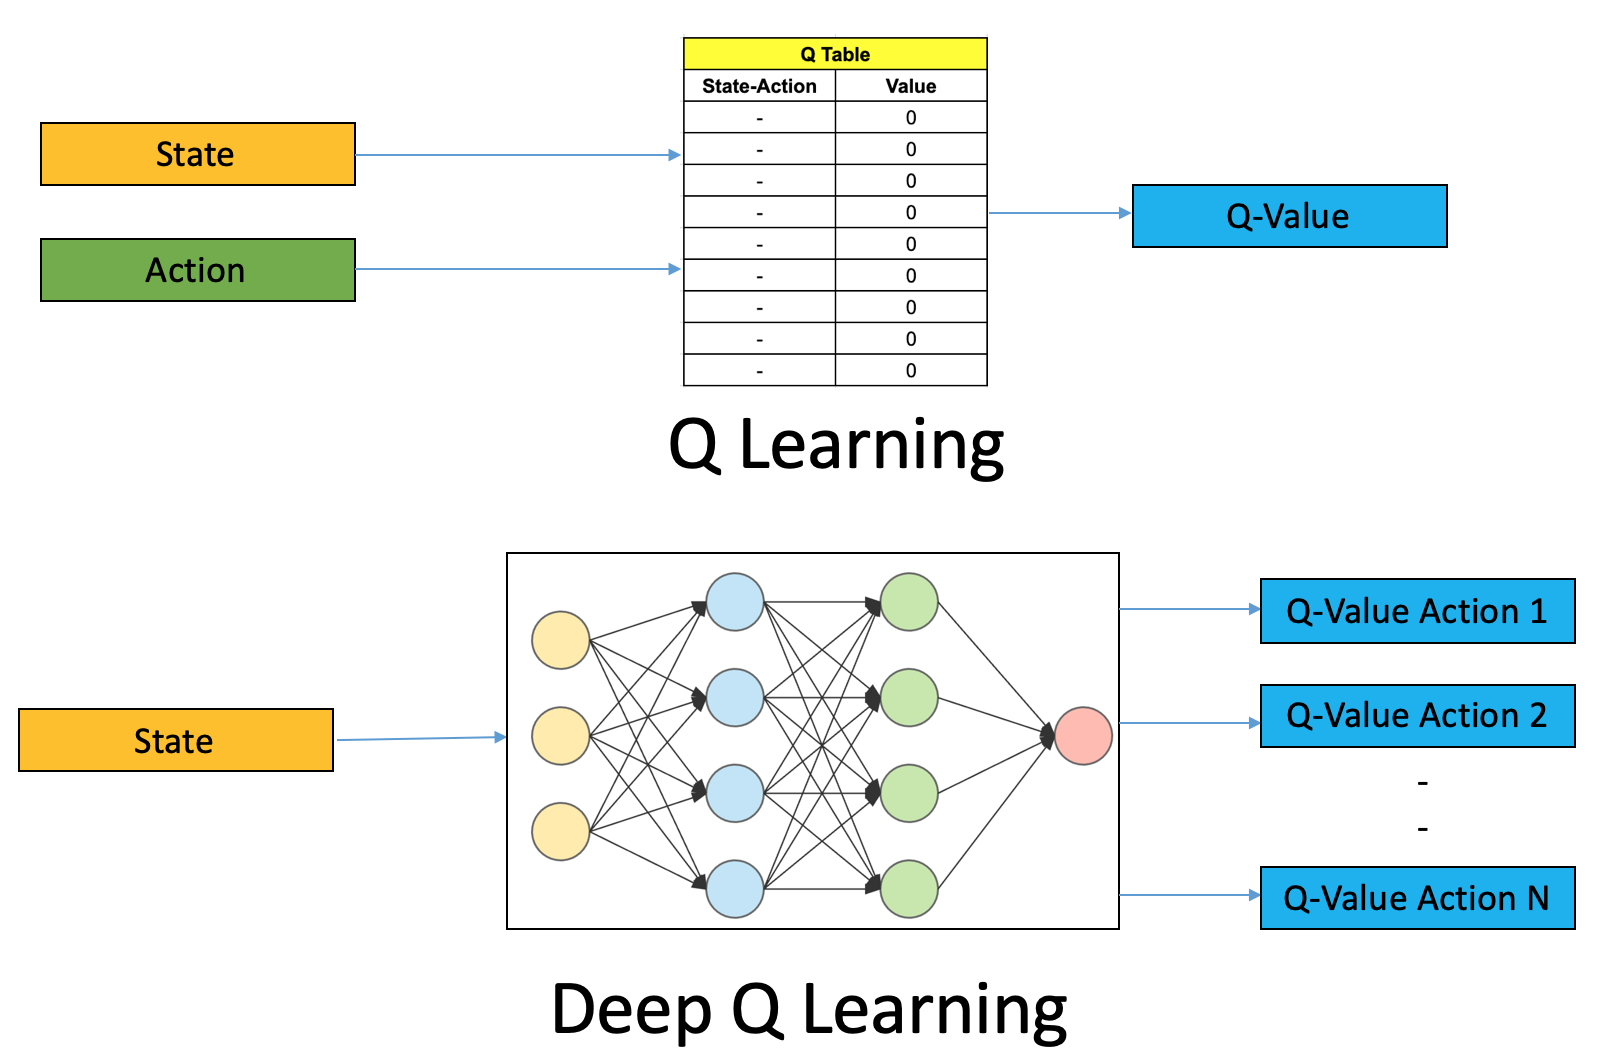
\includegraphics[width=\textwidth]{images/DQN.png}
  \caption{Deep Q Learning architecture comparison with Q-table from \cite{dqnimage}} \label{dqnvsqtable}
\end{figure}

The proposed ANN in \cite{DQN} is a CNN that can be defined by its weights, $\theta_i$, at each iteration. To solve the instability and divergence issues found when using a non-linear function approximator of the action-value function, two methods are proposed. Because these issues arise from the correlations present in the sequence of observations, the paper first proposes a biologically inspired mechanism termed experience replay that collects samples from interaction with the environment in a replay buffer, $U(D)$, and samples randomly from it for training. The second method is an iterative update policy that only adjusts the target weights, $\theta_i^-$, to the new computed weights, $\theta_i$ every $C$ steps.

Since we are dealing with reinforcement learning the loss function of these ANN can not be derived directly from the difference between the expected true value and output, like with supervised learning. Instead we can calculate the loss function according to:
\begin{equation}
    L_i(\theta_i) = E_{(s_t, a_t, r_t, s_{t+1})\sim U(D)} [(r+\gamma \max\limits_{a_{t+1}} Q(s_{t+1}, a_{t+1};\theta_i^-) - Q(s_t, a_t; \theta_i))^2]
\end{equation}

Where the loss, $L_i$, of iteration, $i$, can be calculated by uniformly sampling a mini-batch of experiences from $U(D)$ and calculating the expected value from the difference between our target $t_i=r+\gamma\max\limits_{a_{t+1}} Q(s_{t+1}, a_{t+1};\theta_i^-)$, calculated according to the non-updated weights, $\theta_i^-$, and the resulting action-value predicted by our model.

The gradient can then be calculated by:
\begin{equation}
\nabla L_i(\theta_i) = E [(r+\gamma \max\limits_{a_{t+1}} Q(s_{t+1}, a_{t+1};\theta_i^-) - Q(s_t, a_t; \theta_i))\cdot\nabla Q(s, a;\theta_i)]
\end{equation}

And popular training methods of ANN using gradient descent can be used.

\subsection{Double Deep Q-Network (DDQN)}
\noindent Another proposed method to try to solve the correlation issues present with \acrshort{DQN}s is the idea presented in \cite{doubleDQN} of maintaining two action-value estimation networks, $Q^A$ and $Q^B$. Where in \cite{DQN} the loss is calculated according to a target computed with the maximal valued action of a frozen network, $\theta_i^-$, in paper \cite{doubleDQN} it is proposed that at each update step of one of the networks, the target, $t_i$, must be calculated using the maximal valued action of the other network.

\begin{equation}
    t_i^A = r+\gamma\max\limits_{a_{t+1}}Q^B(s_{t+1}, a_{t+1})
\end{equation}

\begin{equation}
    t_i^B = r+\gamma\max\limits_{a_{t+1}}Q^A(s_{t+1}, a_{t+1})
\end{equation}

This coupled with different experience sets for training each network results in a decoupling from action selection and its evaluation. For picking the next action, the average of the two Q values is calculated in order to evaluate its quality.

\subsection{Prioritized experience replay}
\noindent Improving on the concept of experience replay introduced in paper \cite{DQN}, paper \cite{prioexperience} proposes a way of prioritizing the experience replay buffer, $U(D)$, in order to make the algorithm more efficient and effective. The main component of prioritized experience replay is the criterion used to measure the importance of each experienced transition and as proposed in \cite{prioexperience} the \acrshort{TD}-error, $\delta$, between the target, $t_i$, and the predicted value $Q(s_t,a_t)$ can be used as a proxy for how unexpected the transition is.

With this \acrshort{TD}-error, $\delta$, a greedy \acrshort{TD}-error prioritization algorithm can be devised where experiences for the update step are sampled from the $U(D)$ in order of the highest absolute \acrshort{TD}-error first. This is done with the caveat that new transitions without a known \acrshort{TD}-error are prioritized above all other experiences in order to guarantee that all experiences are seen at least once.

This greedy \acrshort{TD}-error prioritization algorithm comes with several problems. First, in order to avoid recalculating \acrshort{TD} errors for the entire replay memory, they are only updated on replayed transitions. This has the consequence that transitions with low \acrshort{TD} error at first might not be replayed in a long time and due to the limited size of the replay buffer and its sliding window nature, might never be replayed. Other problems with this algorithm is its sensitivity to noise spikes and its tendency to over-fit on a small subset of transitions that have high initial \acrshort{TD}-error.

To solve these issues, the authors of \cite{prioexperience} present a stochastic sampling method that interpolates between pure greedy prioritization and uniform random sampling. To achieve this, they propose that sampling on $U(D)$ be made according to a sampling probability of each transition $i$ defined as:
\begin{equation}
    P(i) = \frac{p_i^\alpha}{\sum_k p_k^\alpha} ,
\end{equation}

where $p_i>0$ is the priority of transition $i$ and $\alpha$ is an hyper-parameter that determines how much prioritization should be used, with $\alpha = 0$ corresponding to the uniform sampling case.

The priority of transition can be defined as:
\begin{equation}
    p_i = |\delta_i|+\epsilon ,
\end{equation}

where $\delta_i$ is the \acrshort{TD}-error of transition $i$ and $\epsilon$ is a small positive constant that prevents edge-cases of transitions not being revisited once their error reaches zero.

An alternative formulation of the priority of transition is:

\begin{equation}
    p_i = \frac{1}{rank(i)} ,
\end{equation}

where $rank(i)$ is the rank of transition $i$ when the replay memory is sorted in descending order according to transition \acrshort{TD}-errors, $|\delta_i|$. This variant is more likely to be more robust because it is insensitive to outliers.

\subsection{Dueling Deep Q-Network (Dueling DQN)}
\noindent Improving upon the concept of double Q-learning presented in \cite{doubleDQN}, the authors of \cite{duelingDQN} present an alternative architecture that tries to explore the insight that for many states, the action taken does not affect what happens. The idea is then to separate the single stream architecture of \cite{DQN} into two streams that estimate the value, $V(s)$, and advantage, $A(s,a)$, functions respectively. A diagram showcasing this split is shown in Figure \ref{duelDQNImag}. 

The value function, $V(s)$, as stated in Equation (\ref{Vfunction}) indicates the expected cumulative reward from beginning in state s and following the policy, $\pi$, and the action-value, $Q(s,a)$, indicates how good is an action, $a$, given the state, $s$. Then, the advantage, $A(s,a)$, can be defined as:

\begin{equation}\label{Qfunction}
Q(s,a) = V(s)+A(s,a) .
\end{equation}

This means which advantage does the agent gain from taking action, $a$, in state, $s$. 

As shown in \cite{duelingDQN}, special consideration must be taken when designing the final aggregating module to output $Q$. A simple aggregation module like the one presented in Equation (\ref{Qfunction}), would make the $V(s)$ inseparable from the $A(s, a)$. So the authors propose an alternative module that forces the advantage function estimator to have zero advantage at the chosen action:

\begin{equation}
    Q(s,a;\theta,\alpha,\beta) = V(s; \theta, \beta) + (A(s,a;\theta,\alpha) - \frac{1}{|A|}\sum\limits_{a'}A(s, a'; \theta, \alpha)) ,
\end{equation}

where $\alpha$ and $\beta$ are hyper-parameters of each stream of fully-connected layers, $A(s,a)$ and $V(s)$ streams respectively and $\theta$ are the weights of the network.

By exploiting the insight that some actions do not affect the state value, this architecture allows the $V(s)$ function to be learned more efficiently and faster resulting in faster convergence of the agent to an optimal policy.

\begin{figure}[H]
  \centering
  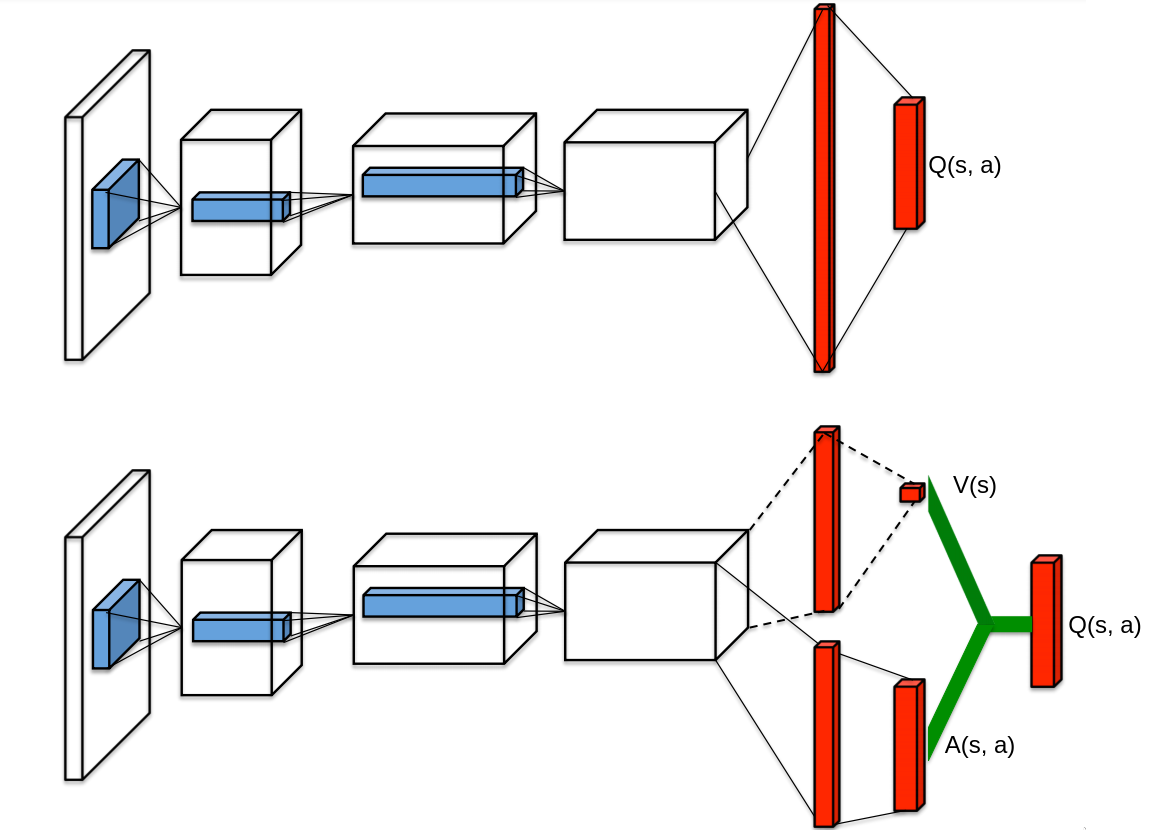
\includegraphics[width=\textwidth]{images/duelingDQN.png}
  \caption{Dueling DQN architecture (bottom) comparison with normal DQN (top), taken from \cite{duelingDQN}} \label{duelDQNImag}
\end{figure}

\subsection{Asynchronous Advantage Actor-Critic (A3C)}\label{A3C}
\noindent Actor-critic methods try to combine the benefits of both value-iteration methods, like Q-learning and policy-iteration methods, like Policy Gradient by separating the agent as an actor network and a critic network. The actor network contains the policy that maps states to actions by a set of parameters $\theta$. While the critic network evaluates the value function $V(s)$, the action-value $Q(s,a)$ or the advantage of an action $A(s,a)$ and based on the \acrshort{TD}-error updates both the actor network and itself. In the case of the \acrshort{A3C}, presented in \cite{a3c}, the critic network tries to estimate the $V(s)$ and the actor network tries to estimate the policy, $\pi(s)$ by maintaining a common network with two streams like in the case of \acrshort{Dueling DQN}, \cite{duelingDQN}. A diagram showcasing the A3C architecture is shown in Figure \ref{A3CImag}.

The gradient of the loss function can then be defined as:
\begin{equation}
    \nabla L(\theta) = \nabla_{\theta'} log_\pi(a_t|s_t; \theta')A(s_t, a_t; \theta, \theta_v) .
\end{equation}

Advantage can be defined as in Equation (\ref{Qfunction}), by using the relationship between the $Q$ and the $V$ functions from the Bellman optimality equation we can get:

\begin{equation}
    Q(s_t, a_t) = E[r_{t+1} + \gamma V(s_{t+1})] ,
\end{equation}

\begin{equation}
    A(s_t, a_t; \theta, \theta_v) = \sum\limits_{i=0}^{k-1} \gamma^i r_{t+i} + \gamma^k V(s_{t+k}; \theta_v) - V(s_t;\theta_v),
\end{equation}

where $k$ is the number of steps used to the compute new update and $\gamma$ is the discount-rate. This bypasses the need for multiple neural networks as $Q$ and $V$ function approximators.

\begin{figure}[h]
  \centering
  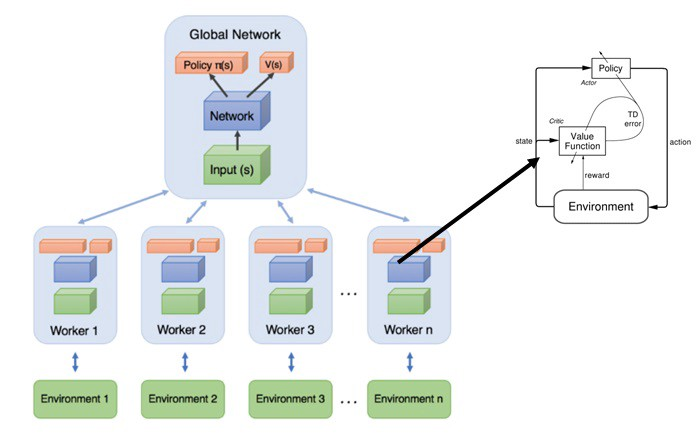
\includegraphics[width=\textwidth]{images/A3C.png}
  \caption{Asynchronous Advantage Actor-Critic (A3C) architecture, taken from \cite{A3CImag}} \label{A3CImag}
\end{figure}

The main difference between the \acrshort{A3C} method and the alternative \acrfull{A2C} method proposed in \cite{openaia2c} and \cite{a2c} is that in \acrshort{A3C} each worker works independently from other workers running $k$ number of experiences and then computing the gradient and updating with a central network asynchronously, where as in \acrshort{A2C} there is a synchronization step where each worker waits for all workers to finish their segments of experience and compute their gradient before updating the central network. Also of note, the authors of the \acrshort{A2C} architecture tested if the distributed asynchronous nature of the \acrshort{A3C} network gave it better performance given the stochastic nature of its updates but found no such advantage. The \acrshort{A2C} method runs more effectively when using single \acrshort{GPU} machines, which perform best on large batch sizes of similar computations.


\section{Exploitation vs Exploration} \label{section:EE}
\noindent One major challenge a \acrshort{RL} agent faces is the exploration vs exploitation dilemma. Given a fixed set of resources that must be allocated between competing choices in a way that maximizes expected reward in an unknown transition probability and reward signal environment, the agent must choose to perform actions that exploit known strategies versus performing unknown actions to explore the environment for better strategies. These types of problems have been studied extensively as multi-armed bandit problems.

\subsection{$\epsilon$-greedy algorithm}
\noindent The most common algorithm used to solve this dilemma is the $\epsilon$-greedy algorithm in which the agent performs a greedy selection of the best action most of the times with a $\epsilon$ probability of choosing a random action.

The best action, in the case of a Q-learning algorithm, can be defined as:

\begin{equation}
    a^* =\arg\max\limits_{a} Q(s, a).
\end{equation}

Where in the case of an actor-critic method like A3C, it can be defined as:

\begin{equation}
    a^* =\arg\max\limits_{a} A(s, a).
\end{equation}

To guarantee sufficient exploration in the beginning versus convergence of the \acrshort{RL} agent policy in the end of training usually the $\epsilon$ value shrinks as training goes on. This reflects the intuition that as training goes on the model becomes better at understanding the environment and the effects of its actions which in turn makes the need to explore less important.

\subsection{Boltzmann exploration} \label{boltz}
\noindent As explained in paper \cite{boltz}, the Boltzmann exploration policy is widely used in \acrshort{RL} problems. The main idea of this algorithm is to build a Boltzmann distribution where instead of using the state's energy, we use the evaluation of the quality of an action, $Q(s,a)$, in the case of Q-learning algorithms or its advantage, $A(s,a)$, in the case of the \acrshort{A3C} algorithm. The probability of choosing each action can be defined according to:

\begin{equation}
    p_i = \frac{e^{-\varepsilon_i/\tau}}{\sum\limits_{j=1}^M e^{-\varepsilon_j/\tau}},
\end{equation}

where $\varepsilon$ is the value of the action, $M$ is the total number of actions and $\tau$ is an hyper-parameter usually called temperature that defines a spectrum between picking the optimal action or a completely random action. When the $\tau$ parameter is close to zero the Boltzmann policy becomes like the greedy policy, picking the highest valued action. Instead, when the $\tau$ parameter is high the probability is more widely distributed between other actions. 

As with the $\epsilon$-greedy, this $\tau$ parameter usually shrinks as training goes on, reflecting the intuition that exploration becomes less important as the agent learns the environment.

\subsection{Adaptive Genetic Algorithm (AGA)} \label{AGA}
\noindent In \acrshort{RL} problems with high-dimensional action spaces, methods like the $\epsilon$-greedy policy are very inefficient in their exploration of the environment. To address this problem the authors of \cite{AGAcrypto}, propose an \acrfull{AGA} to make optimal policy convergence faster by reducing useless exploration without reducing performance.

The main idea behind \acrshort{AGA} is to try to use the critic network to evaluate expected reward for each state-action. The presented solution in \cite{AGAcrypto} is a Q actor-critic architecture where the \acrshort{AGA} takes as input the output action from the actor network. A diagram for the proposed architecture can be seen in Figure \ref{AGAcryptoImag}.

If the loss of the critic network is larger than a defined hyper-parameter, $\varphi$, it is assumed that the critic network cannot evaluate actions very well so a random action is generated. This $\varphi$ hyper-parameter can be set as the convergence loss obtained by pre-training the critic network.

\begin{figure}[h]
  \centering
  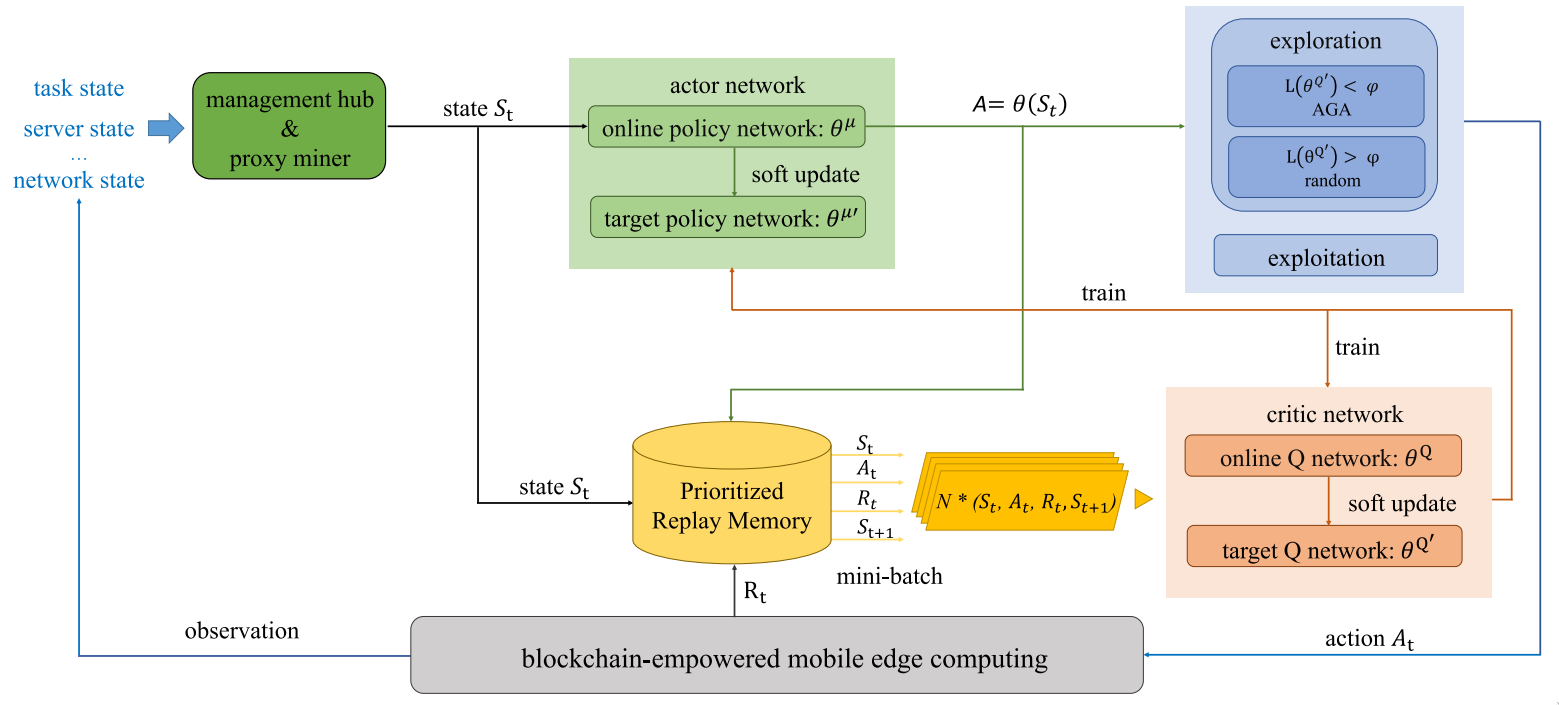
\includegraphics[width=\textwidth]{images/AGA.png}
  \caption{Actor-critic with AGA from \cite{AGAcrypto}} \label{AGAcryptoImag}
\end{figure}

When the critic network can evaluate the state-action pairs, the \acrshort{AGA} works by taking the output action, $A$, from the actor network and generating $m-1$ random actions obtaining a population of candidate solutions of size, $m$. The genetic operators of crossover and mutation can then be used to create different generations of candidates using the critic network evaluation in roulette wheel genetic selection.

The crossover and mutation genetic operators are applied according to their respective probabilities $p_c$ and $p_m$.
\begin{equation}
  p_c =
    \begin{cases}
      \frac{k_1(R_{min}-R')}{\overline{R} - R_{min}} & R' \leq R_{min}\\
      k_3 & R' > R_{min}
    \end{cases},
\end{equation}

\begin{equation}
  p_m =
    \begin{cases}
      \frac{k_2(R-R_{min})}{\overline{R} - R_{min}} & R \geq R_{min}\\
      k_4 & R < R_{min}
    \end{cases},       
\end{equation}

where $\overline{R}$ and $R_{min}$ are the average and minimum value of the population respectively. These parameters are used to make $p_c$ and $p_m$ increase when the population converges to a local minimum. To combat disruptions in the global minimum solution, $p_c$ should depend on its parent action value $R'$ and $p_m$ should depend on the value of the mutating action. $k1$, $k2$, $k3$ and $k4 < 1$ are hyper-parameters that define how much crossovers and mutations should happen.

\acrshort{AGA} ends when a $K$ number of iterations are reached and the highest valued action, $A^*$, is selected. This $K$ value can be adapted by:

\begin{equation}
  K =
    \begin{cases}
      \max(0, K-1) & A^* = A\\
      \min(K + \phi(||A-A^*||_2 ), K_{max}) & A^* \neq A
    \end{cases}.
\end{equation}

Where $\phi$ is a strictly monotonically increasing function and $K_{max}$ is an upper limit on the number of generations. 

\section{Related work} \label{section:RW}

\noindent In order to understand the state of the art in solving \acrshort{MEC} challenges using \acrshort{RL}, several works were reviewed. Their problem statements and solutions are summarized in the following sections.

\subsection{User side task offloading}
\noindent Research papers such as \cite{taskclass1}, \cite{taskclass2} present a local offloading decision algorithm that considers a 1 \acrshort{UE} to 1 \acrshort{MEC} server topology in a 4G environment, where the \acrshort{UE} has information about the required computation graph of its application and makes decisions on which computations to offload and which computations to execute locally. 

In \cite{taskclass1}, the algorithm takes a sequentially dependent list of application computation components  and classifies each one as local or remote execution. It assumes that each component input data amount depends on the output data of the component preceding it and tries to estimate its work as a function of input data and computation complexity as presented in:

\begin{equation} 
    W_c = V \cdot O_n \cdot d_{c-1, c}, 
\end{equation}\label{wcv}

where $W_c$, is the \acrshort{CPU} clock cycles of computation component ($c_n$), V denotes the number of clock cycles a processor will perform per byte, $O_n$ is the computation complexity of $c_n$ and $d_{c-1,c}$ is the output data amount of the previous component.

This paper takes into account the time required to do the computation locally, the transfer delay of uploading input data to \acrshort{MEC} server defined in Equation (\ref{uploaddelay}) and the transfer delay of the downloading of output data defined in Equation (\ref{downloaddelay}):

\begin{equation}\label{uploaddelay}
r_u = n \frac{B}{N} log_2(1+\frac{p_u|h_{ul}|^2}{\Gamma(g_{ul})d^\beta N_0}),
\end{equation}

\begin{equation}\label{downloaddelay}
r_d = n \frac{B}{N} log_2(1+\frac{p_d|h_{dl}|^2}{\Gamma(g_{dl})d^\beta N_0}),
\end{equation}

where B is the bandwidth, $\beta$ is the path loss exponent, $d$ is the distance between the \acrshort{UE} and the \acrshort{MEC} server, $n$ is the number of sub carriers that are allocated for the transmission, $N_0$ is the noise power, $p_u$ and $p_d$ are the transmit powers, $h_{ul}$ and $h_{dl}$ are the channel fading coefficient for uplink and downlink, and $g_{ul}$ and $g_{dl}$ are the required bit error rate for the uplink and downlink. The SNR margin, $\Gamma$, required to satisfy the bit error rate ($g_{ul}$ and $g_{dl}$) with quadrature amplitude modulation constellation can be calculated according to:
\begin{equation} \label{SNR}
    \Gamma(g_{l}) = \frac{-2log5g_{ul}}{3} .
\end{equation}

Data is only transferred as it is needed. This means that when two sequential components are offloaded to the \acrshort{MEC} server, the output of the first component is needed as input for the second component but because they were both computed on the same machine there are no upload or download delays between the two.

The proposed classification algorithm is a Deep Neural Network (DNN) trained using the exhaustively computed best solutions from 10,000 randomly generated states for an application consisting of 100 sequential components. This training method quickly becomes intractable for higher complexity problems.

This work does not take into account energy costs of transmission, idle energy costs of waiting for remote computation execution, assumes sequential data dependency in the execution graph and constant \acrshort{CPU} allocation from the \acrshort{MEC} server. 

\subsection{Centralized Fog Network managers}
\noindent Paper \cite{centralfog}, presents a centralized \acrfull{SDN} controller which maintains global knowledge of the network of fog nodes. Each of these fog nodes receive requests from \acrshort{UE}s and the \acrshort{SDN} controller decides if these tasks should be computed on the receiving node or offloaded to a neighboring node.

This problem statement is formalized as an \acrshort{MDP}, consisting of a state space (S), action space (A), transition probability distribution (P) and a reward (R).

\begin{itemize}
    \item $S = \{s=(n^l, w, Q)\}$ is the state space:
    \begin{itemize}
        \item $n^l \in \mathbb{N}$ $(1\leq n^l \leq N)$, is the fog node requested for tasks by end users;
        \item $w \in \mathbb{N} (1 \le w \le W_{max})$, is the number of requested tasks per unit time;
        \item $Q = \{(Q_1,...,Q_N)|Q_i\in\{0, 1,...,Q_{i,max}\}$, is the number of tasks in the node's queue.
    \end{itemize}
    \item $A = \{a=(n^0, w^0)\}$ is the action space:
    \begin{itemize}
        \item $n^0 \in \mathbb{N}$ $(1 \le n^0 \le N, n^0 \ne n^l)$, is a neighboring node to which node $n^l$ is going to offload to;
        \item $w^0 \in \mathbb{N}$ $(1 \le w^0 \le W_{max})$, is the number of tasks to be offloaded to the neighboring node $n^0$. A node can only offload to nodes with an equal or less number of tasks currently requested. The tasks not offloaded are computed locally ($w^l)$.
    \end{itemize}
    \item $P:S \times A \times S \rightarrow [0, 1]$, is the transition probability distribution $P(s'|s,a)$ of a new state $s'$ given that the system is in state $s$ and action $a$ is chosen.
    \item $R:S\times A \rightarrow \mathbb{R}$, is the reward of the system in state $s$ and action $a$ is taken.
    \begin{itemize}
        \item $R(s,a) = U(s, a) - (D(s,a) + O(s,a))$:
        \begin{itemize}
            \item $U(s, a) = r_u log(1+w^l + w^0)$, is the immediate utility and where $r_u$ is a utility reward;
            \item $D(s,a) = \chi_{d} \cdot \frac{t^w + t^c + t^e}{(w^l + w^0)}$ , is the immediate delay and where $t^w$is the average wait time at queue of node $n^l$ and the node $n^0$, $t^c$ is the communication delay between nodes and $t^e$ is the execution time by node $n^l$ and  $n^0$. The $\chi_d$ is an hyper-parameter that defines importance of the delay;
            \item $O(s, a) = \chi_{0} \cdot \frac{w^l \cdot P_{overload, l} + w^0 \cdot P_{overload, 0}}{w^l + w^0}$, is the overload probability and where $\chi_{0}$ is an overload weight hyper-parameter and $P_{overload, i}$ is the task arrival rate at node.
        \end{itemize}
    \end{itemize}
\end{itemize}

To solve this \acrshort{MDP}, the authors of this work propose a Q-table approach using the $\epsilon$-greed algorithm as its policy, which makes its solution not very scalable to higher dimensional problems and makes it suffer from action value overestimation in noisy environments.

This work does not take into account the possibility of local \acrshort{UE} task execution and associated battery and computation constrains nor the delay in returning computation results from fog nodes back to user device.  It also assumes independence between tasks. Despite mentioning the possibility of software defined fog nodes to be composed by many heterogeneous devices this is not explored.


\subsection{Decentralized Fog Network managers}
\noindent Paper \cite{fogmulti}, continuous the work of paper \cite{centralfog} by introducing a new architecture with two important concepts. First, it introduces the notion of dividing the computation resources of fog nodes into network slices, allowing for the allocation of certain slices to services with specific latency and resource requirements. The second important change it makes in its architecture is the change from a centralized \acrshort{SDN} controller with knowledge of the entire network conditions to many distributed controllers located at each fog node working together.

This new problem can be formulated as a \acrfull{POMDP} in which each fog node only knows its local state and makes decisions on which tasks to offload, where to offload them and how to allocate local slices resources to queued tasks. By doing this no state messages are sent between fog nodes and only locally computed rewards are shared between them. This reward messages can be shared asynchronously from the decision process.

As a solution, each fog nodes has a \acrfull{DRQN} that takes as input a local observation stack of the previous 4 observations and makes a local offloading and resource allocation decision. A variation of the $\epsilon$-greedy algorithm is used in which the $\epsilon$ is reset to the starting value with a small decay $\delta^\epsilon$ $(0<\delta^\epsilon < 1)$ every $R^\epsilon$ steps to solve the insufficient exploration in large state-action spaces that $\epsilon$-greedy algorithm suffers from. These neural networks are trained with the experience replay technique trying to maximize the total system reward composed of the local fog node rewards resulting from their localized actions and their effect on the system as a whole.

The authors of \cite{Lulu}, build on the work done in \cite{fogmulti} by substituting the fog node's \acrshort{DRQN}s by an \acrshort{A2C} architecture with an actor for each network but a common critic estimator for all agents. This critic needs to be updated with all actions and states from each of the fog nodes but can do so asynchronously from the decision process.

\subsection{Centralized MEC controller}
\noindent Finally, the authors of \cite{NUE1mec} present a central decision algorithm that makes offloading and resource allocation decisions between a network of \acrshort{UE}s and 1 \acrshort{MEC} server in a 5G network environment. The algorithm takes as input a list of all tasks that need to be computed by \acrshort{UE}s at that time step and makes a decision of which tasks should be computed on the \acrshort{UE} and which should be offloaded to the \acrshort{MEC} server. It also decides how much of the \acrshort{MEC} server's computation power should be allocated to each offloaded task.

It assumes that each \acrshort{UE} $n$ has a computation-intensive task $R_n \triangleq (B_n, D_n, \tau_n)$ at each time step to be executed, where $B_n$ represents the input data for the computation, $D_n$ represents the total number of \acrshort{CPU} cycles required to compute the task and $\tau_n$ represents the maximum delay amount of that task.

This decision takes into account the delay and energy costs of computing locally, the delay of transmission to \acrshort{MEC} server, the energy needed to transmit and the idle energy consumption of the \acrshort{UE} when waiting for the remote computation. Due to the assumption of very high download rate and smaller size output data than input data, this work ignores the delay and energy cost of downloading the processed result from the \acrshort{MEC} server to the \acrshort{UE}. To solve the problem statement, the authors present a simple \acrshort{DQN}.